\documentclass[a4paper, 12pt]{article}
\usepackage[left=1.8cm,right=1.8cm,top=2cm,bottom=2cm]{geometry}

\usepackage[T1]{fontenc}
\usepackage[utf8]{inputenc}
\usepackage{etex,amsfonts,amssymb,amsmath,mathrsfs}
\usepackage{dsfont}
\usepackage{pifont}
\usepackage[tikz]{bclogo}
\usepackage{tikz,tkz-tab}
\usetikzlibrary{arrows,shadows,shapes,backgrounds,positioning,lindenmayersystems}
\usepackage{fancyhdr}
\usepackage{fancybox}
\setlength{\headheight}{12.81pt}
\usepackage[french]{babel}
\DecimalMathComma
\frenchbsetup{StandardLists=true}
\usepackage{lmodern}
\usepackage{xspace}
\usepackage[francais]{layout}
\usepackage{textcomp} %Pour simple quote droit \textquotesingle
\usepackage{fourier-orns}
\usepackage{colortbl}
\usepackage{multicol}
\usepackage{multirow}
\usepackage{numprint}
\usepackage{multido}
\usepackage{ifthen}
%%%%%%%%%%%%%%%%%%%%%%%%%%%%%%%%%%%%%%%%%%%%%%%%%%%%%%%%%%%%%%
\usepackage[french,lined,vlined,linesnumbered]{algorithm2e}
% \usepackage[french,lined,vlined,linesnumbered,boxed]{algorithm2e}
\setlength{\algomargin}{1em}
%%%%%%%%%%%%%%%%%%%%%%%%%%%%%%%%%%%%%%%%%%%%%%%%%%%%%%%%%%%%%%
\usepackage{stmaryrd}
\SetSymbolFont{stmry}{bold}{U}{stmry}{m}{n}
\usepackage{alltt}
\usepackage{moreverb}
\usepackage{appendix}

%%%%%%%%%%%%%%%%%%%%%%%%%%%%%%%%%%%%%%%%%%%%%%%%%%%%%%%%%%%%%%
%%%%%%%%%%%%%%%%%%%%%%%%%%%%%%%%%%%%%%%%%%%%%%%%%%%%%%%%%%%%%%

\usepackage{cellspace}
% Pour régler l'espacement vertical des filets et du texte dans un tableau
% \cellspacetoplimit=3pt
% \cellspacebottomlimit=3pt
% écrire Sc pour une colonne centrée

%%%%%%%%%%%%%%%%%%%%%%%%%%%%%%%%%%%%%%%%%%%%%%%%%%%%%%%%%%%%%%
%%%%%%%%%%%%%%%%%%%%%%%%%%%%%%%%%%%%%%%%%%%%%%%%%%%%%%%%%%%%%%

\graphicspath{{images/}}

%%%%%%%%%%%%%%%%%%%%%%%%%%%%%%%%%%%%%%%%%%%%%%%%%%%%%%%%%%%%%%
%%%%%%%%%%%%%%%%%%%%%%%%%%%%%%%%%%%%%%%%%%%%%%%%%%%%%%%%%%%%%%

% \renewcommand{\textbf}[1]{\begingroup\bfseries{\mathversion{bold}#1}\endgroup}
\usepackage{varwidth} 
\usepackage{setspace}
\usepackage{amsmath}
\usepackage{fancybox, graphicx}
\pagestyle{fancy}
\renewcommand{\footrulewidth}{1pt}
\fancyfoot[L]{La Pr\'epa des INP - Bordeaux}
\fancyfoot[C]{\thepage}
\fancyfoot[R]{Ann\'ee universitaire 2019-2020}
\fancyhead[L]{\leftmark}
\fancyhead[C]{}
\fancyhead[R]{Ondes acoustiques dans les fluides}

\begin{document}

\begin{titlepage}
{
\includegraphics[height=1.5cm]{bx-inp.png}}
{
\includegraphics[height=1.5cm]{cpp-inp.png}}
\vspace*{\stretch{1}}
\begin{center}
 \Huge{\textbf{Cours d'ondes acoustiques dans les fluides}}
\end{center}
\vspace*{\stretch{0.25}}
\begin{center}
 \normalsize{Axel MATAVAR - Alexandre CHOURA - Etienne LEMESLE}
\end{center}
\vspace*{\stretch{0.25}}
\begin{center}
 {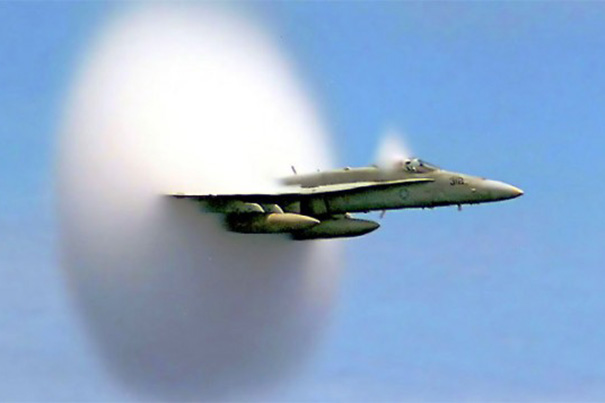
\includegraphics[scale=0.65]{frst-pg.png}}
\end{center}
\vspace*{\stretch{1}}
\begin{center}
 \Large{\textit{Ann\'ee universitaire 2019-2020}}
\end{center}
\vspace*{\stretch{1}}
\end{titlepage}

\tableofcontents
\newpage

\section{Mise en équation des ondes sonores}

\newpage
\section{Ondes sonores planes progressives}

\newpage
\section{Aspects énergétiques}

\newpage
\section{Ondes sonores stationnaires}

\subsection{Énergie d'une onde stationnaire}

\begin{itemize}
\item Pour une onde stationnaire, les variations spatiales et temporelles sont découplées. Une onde sonore stationnaire prend naissance dans des milieux matériels qui limitent la propagation à un domaine fini de l'espace. Ces limites spatiales imposent des conditions aux limites sur les champs de surpression $p$ et de vitesse $\overrightarrow{v}$. 
\end{itemize}

\textit{Écriture}

\noindent\shadowbox{\begin{minipage}[t]{1\linewidth}%
\begin{itemize}
\item Sans perte de généralité, on peut envisager l'écriture du champ de vitesse $\overrightarrow{v}$ sous la forme:
\end{itemize}
\begin{center}
\scalebox{1.2}{$\overrightarrow{v}(z,t)=v_{m}\cos(\omega t+\phi)\cos(kz)\overrightarrow{e_{z}}$}
\end{center}
\begin{itemize}
\item Cette expression peut également s'écrire comme la combinaison linéaire de deux OPPH, l'une se propageant dans le sens de $e_{z}$, l'autre en sens opposé:
\end{itemize}
\begin{center}
\scalebox{1.2}{$\overrightarrow{v}(z,t)=\underset{\textrm{sens des z positifs}}{\underbrace{\frac{v_{m}}{2}\cos(\omega t-kz+\phi)\overrightarrow{e_{z}}}}+\underset{\textrm{sens des z négatifs}}{\underbrace{\frac{v_{m}}{2}\cos(\omega t+kz+\phi)\overrightarrow{e_{z}}}}$}
\end{center}
\end{minipage}}

Cette décomposition permet de déterminer le champ de surpression $p$ en utilisant l'expression de l'impédance acoustique pour une OPPH. Ainsi, on obtient:
\begin{center}
\scalebox{1.2}{$p(z,t)=\rho_{0}c\frac{v_{m}}{2}\cos(\omega t-kz+\phi)-\rho_{0}c\frac{v_{m}}{2}\cos(\omega t+kz+\phi)$}
\end{center}

soit:

\begin{center}
\scalebox{1.2}{$p(z,t)=\rho_{0}cv_{m}\sin(\omega t+\phi)\sin(kz)$}
\end{center}

On en déduit le vecteur densité de courant d'énergie $\overrightarrow{\Pi}$ : 
\begin{center}
\scalebox{1.2}{$\overrightarrow{\Pi}=p\overrightarrow{v}=\frac{\rho_{0}cv_{m}^{2}}{4}\sin(2\omega t+2\phi)\sin(2kz)\overrightarrow{e_{z}}$}
\end{center}

dont la valeur moyenne temporelle est nulle:

\begin{center}
\scalebox{1.2}{$\left\langle \overrightarrow{\Pi}\right\rangle =\frac{\rho_{0}cv_{m}^{2}}{4}\sin(2kz)\left\langle \sin(2\omega t+2\phi)\right\rangle \overrightarrow{e_{z}}=0$}
\end{center}

\noindent\shadowbox{\begin{minipage}[t]{1\linewidth}%
\begin{itemize}
\item Une onde sonore stationnaire \textbf{ne transporte pas d'énergie}.
\item  Cependant, cela ne signifie pas que l'énergie sonore est nulle. En effet, un calcul analogue à celui de $\overrightarrow{\Pi}$ donnerait
\end{itemize}
\begin{center}
\scalebox{1.2}{$\left\langle e\right\rangle =\frac{\rho_{0}v_{m}^{2}}{4}$}
\end{center}

\end{minipage}}

\subsection{Ordres de grandeurs}

\begin{itemize}
\item L'onde sonore doit son nom au fait qu'elle est détectable par l'oreille. L'oreille est donc un détecteur sensible aux surpressions. 
\item Les puissances surfaciques audibles varient d'environ $10^{-12}$ $W\cdot m^{-2}$, pour le seuil d'audition, à environ $1$ $W\cdot m^{-2}$. 
\item Le domaine des fréquences audibles varie de $20$ Hz à $20$ kHz. Avec de telles valeurs, il est possible de donner l'ordre de grandeur des surpressions et des vitesses associées à une onde sonore.
\end{itemize}

\noindent\shadowbox{\begin{minipage}[t]{1\linewidth}%
\begin{itemize}
\item Ainsi, pour une OPPH de pulsation $\omega$, l'amplitude $v_{m}$ de la vitesse des particules fluides (en $m\cdot s^{-1}$), l'amplitude $x_{m}$ du mouvement des particules fluides (en $m$) et l'amplitude $p_{m}$ de la surpression (en Pa) ont respectivement pour expression:
\end{itemize}
\begin{center}
\scalebox{1.2}{$v_{m}=\sqrt{\frac{2\left\langle \Pi\right\rangle }{\rho_{0}c}}$; $x_{m}=\frac{v_{m}}{\omega}$} et \scalebox{1.2}{$p_{m}=\sqrt{2\rho_{0}c\left\langle \Pi\right\rangle }$}
\end{center}
\begin{itemize}
\item De plus, dans le cas d'un gaz parfait, l'amplitude $\rho_m$ de la masse volumique (en $kg\cdot m^{-3}$) vérifie la relation:
\end{itemize}
\begin{center}
\scalebox{1.2}{$\rho_{m}=\rho_{0}\chi_{0}p_{m}=\frac{Mp_{m}}{\gamma RT_{0}}$}
\end{center}
\end{minipage}}

En considérant une OPPH de fréquence $1$ kHz se propageant dans l'air assimilé à un gaz parfait pris à température ambiante ($\rho_{0} = 1.2$ $kg\cdot m^{-3}$, $T_{0} = 298$ $K$), pour une puissance surfacique moyenne égale à $10^{-5}$ $W\cdot m^{-2}$, on calcule les valeurs suivantes:
\begin{center}
$v_{m} = 0.2$ $cm\cdot s^{-1}$; $x_{m} = 3.5\cdot 10^{-8}$ $m$; $p_{m} = 0.1$ Pa; $\rho_{m} = 1\cdot 10^{-6}$ $kg\cdot m^{-3}$
\end{center}

La faible valeur de $x_{m}$ montre combien l'oreille est un détecteur sensible puisque $x_{m}$ est aussi l'amplitude du mouvement du tympan. Ces valeurs permettent également de valider les hypothèses initialement émises dans le cadre de l'approximation acoustique. En effet:
\begin{itemize}
\item La surpression $p$ reste très petite devant la pression $p_{0}$ de l'ordre de $10^{5}$ Pa: $\left|p\right|\ll p_{0}$
\item La masse volumique $\rho$ reste très petite devant $\rho_{0}$: $\left|\rho\right|\ll \rho_{0}$
\item La vitesse $v$ considérée comme "petite", sans autre justification, peut être comparée à la seule vitesse qui caractérise les ondes sonores, à savoir leur vitesse $c$: $v_{m}\ll c$
\end{itemize}

\subsection{Retour sur les hypothèses}

Les résultats précédents permettent également de vérifier la validité des autres hypothèses émises aux début de ce cours. En considérant une OPPH, il s'introduit naturellement:
\begin{itemize}
\item Une échelle caractéristique de longueur, par l'intermédiaire de la longueur d'onde $\lambda$;
\item Une échelle caractéristique de temps, par l'intermédiaire de la période $T$;
\end{itemize}

La longueur d'onde $\lambda$ fournit une échelle de distance de variation des champs $p$, $\rho$ et $v$; la période $T$ fournit une échelle de temps de variation de ces mêmes champs. Ainsi, on peut écrire

\noindent\shadowbox{\begin{minipage}[t]{1\linewidth}%
\begin{center}
\scalebox{1.2}{$\left|\frac{\partial v}{\partial t}\right|\sim\frac{v_{m}}{T}$ ; $\left|\frac{\partial^{2}v}{\partial t^{2}}\right|\sim\frac{v_{m}}{T^{2}}$ ; $\left|\frac{\partial v}{\partial x}\right|\sim\frac{v_{m}}{\lambda}$ ; $\left|\frac{\partial^{2}v}{\partial x^{2}}\right|\sim\frac{v_{m}}{\lambda^{2}}$}
\end{center}
\end{minipage}}

\begin{itemize}
\item Le terme d'accélération convective peut bien être négligé devant le terme d'accélération locale. En effet, on a:
\end{itemize}
\begin{center}
\scalebox{1.5}{$\left\Vert \frac{(\overrightarrow{v}\cdot\overrightarrow{\textrm{grad}})\overrightarrow{v}}{\frac{\partial\overrightarrow{v}}{\partial t}}\right\Vert \sim\frac{v_{m}\cdot\frac{v_{m}}{\lambda}}{\frac{v_{m}}{T}}=v_{m}\frac{T}{\lambda}=\frac{v_{m}}{c}\ll1$}
\end{center}

\begin{itemize}
\item Le terme de pesanteur peut bien être négligé devant le gradient de surpression. En effet, on a:
\end{itemize}
\begin{center}
\scalebox{1.5}{$\left\Vert \frac{\rho\overrightarrow{g}}{\overrightarrow{\textrm{grad}}p}\right\Vert \sim\frac{\rho_{m}g}{\frac{p_{m}}{\lambda}}=\frac{\rho_{0}\chi_{0}p_{m}gc}{p_{m}f}=\frac{gc}{c^{2}f}=\frac{g}{cf}$}
\end{center}

Dans l'air, la vitesse $c$ du son est de l'ordre de $3\cdot 10^{2}$ $m\cdot s^{-1}$. Le rapport calculé reste donc faible devant l'unité pour des fréquences $f$ supérieures à $3$ Hz, condition satisfaite pour les ondes sonores.

\begin{itemize}
\item L'hypothèse adiabatique consiste à considérer l'évolution du phénomène suffisamment rapide pour pouvoir négliger les échanges thermiques entre les particules fluides. Cela revient à comparer le temps caractéristique de diffusion thermique $\tau_{therm}$ au temps caractéristique de variation de la perturbation sonore $\tau_{son}$. En introduisant la taille caractéristique d'une particule de fluide (en $m$) et sa diffusivité thermique $D$ (en $m^{2}\cdot s^{-1}$), on a:
\end{itemize}
\begin{center}
\scalebox{1.2}{$\tau_{therm}=\frac{d^{2}}{D}$} avec \scalebox{1.2}{$D=\frac{\lambda_{m}}{\rho c_{m}}$}
\end{center}

La taille caractéristique d'une particule fluide est celle de la variation du phénomène ondulatoire, i.e. sa longueur d'onde $\lambda$. Quand à $\tau_{son}$, il est donné par la période temporelle $T$ de l'onde.

Dans l'air ($D = 1.87\cdot 10^{-5}$ $m^{2}\cdot s^{-1}$), pour une OPPH de fréquence $1$ kHz, le rapport des temps caractéristiques a pour ordre de grandeur:
\begin{center}
\scalebox{1.2}{$\frac{\tau_{therm}}{\tau_{son}}=\frac{\lambda^{2}}{DT}=\frac{c^{2}}{af}\approx6\cdot10^{6}$}
\end{center}

ce qui justifie l'hypothèse adiabatique.

\newpage
\section{Réflexion et transmission}

\subsection{Conditions aux limites}

\begin{center}
 {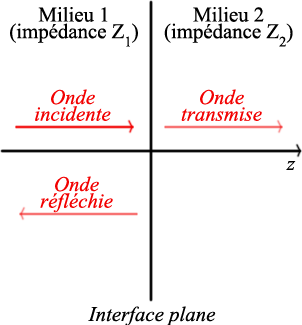
\includegraphics[scale=0.65]{ref_trans.png}}
\end{center}

\begin{itemize}
\item Considérons une interface plane infinie entre deux fluides située en $z=0$. Une onde progressive plane émise dans la région $z < 0$ se propage dans le sens des $z$ croissants vers l'interface. Elle tombe sur l'interface sous incidence normale et elle y est en partie réfléchie et en partie transmise. L'onde réfléchie se propage dans le sens des $z < 0$, l'onde transmise dans le sens des $z > 0$.

\item On note $\overrightarrow{v}_{i}$, $p_{i}$ les champs de vitesse et de surpression associés à l'onde incidente, $\overrightarrow{v}$, $p$, ceux associés à l'onde réfléchie et enfin $\overrightarrow{v}_{t}$, $p_{t}$ ceux associés à l'onde transmise. 



\item Quand l'onde tombe sur l'interface, la composante de la vitesse normale à la surface de séparation entre les milieux est égale à gauche et à droite de celle-ci car les déplacements des fluides y sont les mêmes.

\end{itemize}

\noindent\shadowbox{\begin{minipage}[t]{1\linewidth}%
\begin{itemize}
\item Sous incidence normale, il y a continuité des champs de vitesse à l'interface:
\end{itemize}
\begin{center}
$\overrightarrow{v}_{i}(z=0,t)+\overrightarrow{v}_{r}(z=0,t)=\overrightarrow{v}_{t}(z=0,t)$
\end{center}

\end{minipage}}

\begin{itemize}
\item Dans l'approximation acoustique, l'interface peut être considérée comme fixe, ses déplacements restant faibles devant la longueur d'onde. En appliquant la relation fondamentale de la dynamique à un élément de surface dS de l'interface (de masse nulle), il vient après projection sur l'axe des $z$:
\end{itemize}

\begin{center}
$(p_{0} + p_{i} + p_{r})dS - (p_{0} + p_{t})dS = 0$
\end{center}

Ainsi, il n'existe aucune différence entre les pressions exercées par les fluides de part et d'autre de la surface.

\newpage
\noindent\shadowbox{\begin{minipage}[t]{1\linewidth}%
\begin{itemize}
\item Sous incidence normale, il y a continuité des champs de surpression à l'interface:
\end{itemize}
\begin{center}
$p_{i}(z=0,t)+p_{r}(z=0,t)=p_{t}(z=0,t)$
\end{center}
\end{minipage}}

Pour une OPPH, les différents champs considérés peuvent s'écrire en représentation complexe:
\begin{center}
$\left|\begin{array}{ccc}
\overrightarrow{\underline{v}_{i}} & = & \underline{v}_{im}e^{j(\omega t-k_{1}z)}\overrightarrow{u_{z}}\\
\underline{p}_{i} & = & \underline{p}_{im}e^{j(\omega t-k_{1}z)}
\end{array}\right.\left|\begin{array}{ccc}
\overrightarrow{\underline{v}_{r}} & = & \underline{v}_{rm}e^{j(\omega t-k_{1}z)}\overrightarrow{u_{z}}\\
\underline{p}_{r} & = & \underline{p}_{rm}e^{j(\omega t-k_{1}z)}
\end{array}\right.\left|\begin{array}{ccc}
\overrightarrow{\underline{v}_{t}} & = & \underline{v}_{tm}e^{j(\omega t-k_{2}z)}\overrightarrow{u_{z}}\\
\underline{p}_{t} & = & \underline{p}_{tm}e^{j(\omega t-k_{2}z)}
\end{array}\right.$
\end{center}

\textit{Propriété}

\noindent\shadowbox{\begin{minipage}[t]{1\linewidth}%
\begin{itemize}
\item Pour une OPPH, les \textbf{conditions aux limites à l'interface $(z=0)$} se traduisent par deux relations entre les amplitudes des champs de vitesse et de surpression:
\end{itemize}
\begin{center}
$\begin{cases}
\underline{v}_{im}+\underline{v}_{rm} & =\underline{v}_{tm}\\
\underline{p}_{im}+\underline{p}_{rm} & =\underline{p}_{tm}
\end{cases}$
\end{center}
\end{minipage}}

\subsection{Coefficients de réflexion et de transmission en amplitude}

\begin{itemize}
\item Pour une OPPH, les relations précédentes permettent de caractériser l'interface par son coefficient de réflexion $r_{v}$ et son coefficient de transmission $t_{v}$ en amplitude des vitesses définis en $z = 0$ par:
\end{itemize}
\begin{center}
\scalebox{1.2}{$r_{v}=\frac{\underline{v}_{r}}{\underline{v}_{i}}=\frac{\underline{v}_{rm}}{\underline{v}_{im}}$} et \scalebox{1.2}{$t_{v}=\frac{\underline{v}_{t}}{\underline{v}_{i}}=\frac{\underline{v}_{tm}}{\underline{v}_{im}}$}
\end{center}

En introduisant les impédances acoustiques $Z_{1}$ et $Z_{2}$ des deux fluides, les conditions aux limites s'écrivent:
\begin{center}
$\begin{cases}
\underline{v}_{im}+\underline{v}_{rm} & =\underline{v}_{tm}\\
Z_{1}\underline{v}_{im}-Z_{1}\underline{v}_{rm} & =Z_{2}\underline{v}_{tm}
\end{cases}$
\end{center}

d'où l'on déduit le système:
\begin{center}
$\begin{cases}
1+r_{v} & =t_{v}\\
Z_{1}(1-r_{v}) & =Z_{2}t_{v}
\end{cases}$
\end{center}

\textit{Propriété}

\noindent\shadowbox{\begin{minipage}[t]{1\linewidth}%
\begin{itemize}
\item Pour une OPPH, les coefficients de réflexion $r_{v}$ et de transmission $t_{v}$ \textbf{en amplitude des vitesses}, sous incidence normale, sont à l'interface:
\end{itemize}
\begin{center}
\scalebox{1.2}{$r_{v}=\frac{Z_{1}-Z_{2}}{Z_{1}+Z_{2}}$} et \scalebox{1.2}{$t_{v}=\frac{2Z_{1}}{Z_{1}+Z_{2}}$}
\end{center}
où $Z_{1}$ et $Z_{2}$ sont les impédances acoustiques des deux fluides.
\end{minipage}}

On remarque tout d'abord que ces coefficients sont réels puisque les impédances $Z_{1}$ et $Z_{2}$ le sont. Le coefficient de transmission $t_{v}$ est toujours positif: les ondes incidente et transmise vibrent toujours en phase. Le coefficient de réflexion $r_{v}$ peut être négatif: les ondes incidente et réfléchie vibrent soit en phase, soit en opposition de phase.

En outre, la réflexion est d'autant plus faible et la transmission d'autant plus grande que les impédances des milieux sont proches. Ainsi, si $Z_{1}=Z_{2}$, on a $r_{v} = 0$ et $t_{v} = 1$ : l'onde est totalement transmise, ce qui constitue une situation dite \textbf{d'adaptation d'impédances.}

\textit{A contrario}, si $Z_{2} = \infty$ (cas d'un Milieu 2 de compressibilité nulle), $r_{v} = -1$ et $t_{v} = 0$ : l'onde est totalement réfléchie. De même, si $Z_{2} = 0$ (cas d'un Milieu 2 identique au vide), il ne peut pas y avoir de propagation : l'onde est donc totalement réfléchie.

\textit{Définitions}

\noindent\shadowbox{\begin{minipage}[t]{1\linewidth}%
\begin{itemize}
\item Il est également possible de définir un coefficient de réflexion $r_{p}$ et un coefficient de transmission $t_{p}$ en amplitude des surpressions par:
\end{itemize}
\begin{center}
\scalebox{1.2}{$r_{p}=\frac{\underline{p}_{r}}{\underline{p}_{i}}$} et \scalebox{1.2}{$t_{p}=\frac{\underline{p}_{t}}{\underline{p}_{i}}$}
\end{center}

\begin{itemize}
\item Identiquement aux calculs de $r_{v}$ et $t_{v}$ (les rôles de $Z_{1}$ et $Z_{2}$ étant inversés), pour une OPPH, les coefficients de réflexion $r_{p}$ et de transmission $t_{p}$ \textbf{en amplitude des surpressions}, sous incidence normale, sont à l'interface:
\end{itemize}

\begin{center}
\scalebox{1.2}{$r_{p}=\frac{Z_{2}-Z_{1}}{Z_{1}+Z_{2}}$} et \scalebox{1.2}{$t_{p}=\frac{2Z_{2}}{Z_{1}+Z_{2}}$}
\end{center}

\end{minipage}}

\subsection{Coefficients de réflexion et de transmission en puissance}

\begin{itemize}
\item Il est également possible de caractériser l'interface par des coefficients de réflexion $R$ et de transmission $T$ des puissances sonores qui s'expriment en fonction des puissances surfaciques moyennes incidente $P_{i}$, réfléchie $P_{r}$ et transmise $P_{t}$:
\end{itemize}

\begin{center}
\scalebox{1.2}{$R=\frac{P_{r}}{P_{i}}$} et \scalebox{1.2}{$T=\frac{P_{t}}{P_{i}}$}
\end{center}

\begin{itemize}
\item La puissance surfacique moyenne échangée par l'onde est égale à la valeur moyenne temporelle $\left\langle \Pi\right\rangle$ du vecteur densité de courant d'énergie. On a:
\end{itemize}

\begin{center}
\scalebox{1.2}{$\left\langle \Pi\right\rangle =\frac{\rho_{0}c}{2}v_{m}^{2}$} avec $Z = \rho_{0}c$.
\end{center}

Pour une OPPH, il en vient:
\begin{center}
\scalebox{1.2}{$P_{i}=\frac{Z_{1}}{2}\left|\underline{v}_{im}\right|^{2}$, $P_{r}=\frac{Z_{1}}{2}\left|\underline{v}_{rm}\right|^{2}$ et $P_{t}=\frac{Z_{1}}{2}\left|\underline{v}_{tm}\right|^{2}$}
\end{center}
avec $\underline{v}_{rm}=r_{v}\underline{v}_{im}$ et $\underline{v}_{tm}=t_{v}\underline{v}_{im}$

\textit{Définition}

\noindent\shadowbox{\begin{minipage}[t]{1\linewidth}%
\begin{itemize}
\item Pour une OPPH, les coefficients de réflexion $r$ et de transmission $t$ \textbf{des puissances sonores}, sous incidence normale, s'écrivent:
\end{itemize}
\begin{center}
\scalebox{1.2}{$\begin{cases}
R=r_{v}^{2} & =\left(\frac{Z_{1}-Z_{2}}{Z_{1}+Z_{2}}\right)^{2}\\
T=t_{v}^{2}\frac{Z_{2}}{Z_{1}} & =\frac{4Z_{1}Z_{2}}{(Z_{1}+Z_{2})^{\text{2}}}
\end{cases}$}
\end{center}
Ces coefficients ne sont pas indépendants l'un de l'autre puisque $R+T=1$.
\end{minipage}}

La dernière relation ne fait que traduire la conservation de l'énergie en l'absence de phénomènes dissipatifs: l'énergie incidente est pour une part réfléchie, pour l'autre part transmise.

Comme pour les coefficients en amplitude, une onde sonore est d'autant mieux transmise d'un point de vue énergétique que les impédances des fluides sont proches. Cette propriété est exploitée, par exemple, en échographie médicale. En effet, bien que l'adaptation d'impédances ne puisse être satisfaite, un gel déposé sur le corps assure une meilleure transmission des ondes ultra-sonores.

\textit{A contrario}, il peut également être intéressant de limiter la transmission d'un son, par exemple pour mettre en place un système d'isolation phonique. On travaille alors avec des milieux d'impédances très différentes: un fluide gazeux ($Z$ de l'ordre de $10^{2}$ $kg\cdot m^{-2}\cdot s^{-1}$) et un solide ($Z$ de l'ordre de $10^{6}$ $kg\cdot m^{-2}\cdot s^{-1}$), l'onde sonore incidente prenant naissance dans le gaz. En tombant sur le solide, l'onde est presque totalement réfléchie.

\newpage
\section{Application sous forme d'un exercice}

\begin{doublespace}
Encore un autre paragraphe.
\end{doublespace}

\end{document}